\documentclass{beamer}

% Theme choice
\usetheme{Madrid} % You can change to e.g., Warsaw, Berlin, CambridgeUS, etc.

% Encoding and font
\usepackage[utf8]{inputenc}
\usepackage[T1]{fontenc}

% Graphics and tables
\usepackage{graphicx}
\usepackage{booktabs}

% Code listings
\usepackage{listings}
\lstset{
basicstyle=\ttfamily\small,
keywordstyle=\color{blue},
commentstyle=\color{gray},
stringstyle=\color{red},
breaklines=true,
frame=single
}

% Math packages
\usepackage{amsmath}
\usepackage{amssymb}

% Colors
\usepackage{xcolor}

% TikZ and PGFPlots
\usepackage{tikz}
\usepackage{pgfplots}
\pgfplotsset{compat=1.18}
\usetikzlibrary{positioning}

% Hyperlinks
\usepackage{hyperref}

% Title information
\title{Chapter 11: Ethical Considerations in AI}
\author{Your Name}
\institute{Your Institution}
\date{\today}

\begin{document}

\frame{\titlepage}

\begin{frame}[fragile]
    \frametitle{Introduction to Ethical Considerations in AI}
    \begin{block}{Overview}
        This presentation discusses the significance of ethics in artificial intelligence (AI) and its impact on society.
    \end{block}
\end{frame}

\begin{frame}[fragile]
    \frametitle{Explanation of Concepts}
    \begin{itemize}
        \item \textbf{Ethics in Artificial Intelligence:} 
            Principles guiding the development and deployment of AI technologies, ensuring societal benefits while minimizing harm.
        \item \textbf{Significance of Ethics in AI:} 
            Critical for influencing public trust and impacting societal norms, especially as AI integrates into daily life.
    \end{itemize}
\end{frame}

\begin{frame}[fragile]
    \frametitle{Examples Illustrating Ethical Concerns}
    \begin{enumerate}
        \item \textbf{Autonomous Vehicles:} 
            Ethical dilemmas arise in programming vehicles for accident scenarios, involving decisions about lives and property.
        \item \textbf{Facial Recognition Technology:} 
            Risks of privacy invasion and discriminatory profiling, particularly when algorithms reflect societal biases.
        \item \textbf{AI in Hiring:} 
            Possibility of embedding biases into recruitment processes, resulting in unfair practices against underrepresented candidates.
    \end{enumerate}
\end{frame}

\begin{frame}[fragile]
    \frametitle{Key Points to Emphasize}
    \begin{itemize}
        \item \textbf{Public Trust:} 
            Ethical AI fosters transparency and accountability, essential for gaining public confidence.
        \item \textbf{Bias and Fairness:} 
            Need to understand and mitigate bias to prevent social inequalities exacerbated by unchecked AI systems.
        \item \textbf{Regulation and Governance:} 
            Importance of establishing regulations to demarcate ethical boundaries for responsible AI innovation.
    \end{itemize}
\end{frame}

\begin{frame}[fragile]
    \frametitle{Ethical AI Framework}
    \begin{center}
        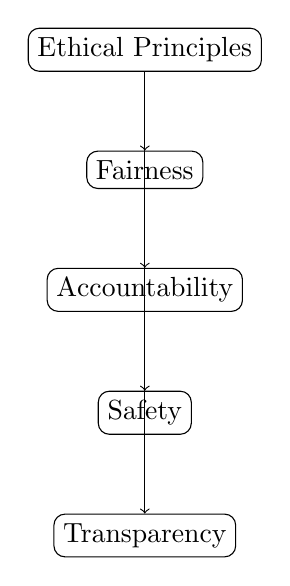
\begin{tikzpicture}
            \node (main) [draw, rectangle, rounded corners] {Ethical Principles};
            \node (fairness) [draw, rectangle, rounded corners, below=of main] {Fairness};
            \node (accountability) [draw, rectangle, rounded corners, below=of fairness] {Accountability};
            \node (safety) [draw, rectangle, rounded corners, below=of accountability] {Safety};
            \node (transparency) [draw, rectangle, rounded corners, below=of safety] {Transparency};

            \draw[->] (main) -- (fairness);
            \draw[->] (main) -- (accountability);
            \draw[->] (fairness) -- (safety);
            \draw[->] (accountability) -- (transparency);
        \end{tikzpicture}
    \end{center}
\end{frame}

\begin{frame}[fragile]
    \frametitle{Summary}
    \begin{block}{Conclusion}
        Ethical considerations in AI are essential for the responsible harnessing of technology. 
        Addressing ethical challenges allows for the leveraging of AI to improve societies while safeguarding against potential harms. 
        Next, we will explore specific ethical issues, such as bias, to better understand their implications.
    \end{block}
\end{frame}

\begin{frame}[fragile]
    \frametitle{Understanding Bias in AI - Definition}
    % Definition of bias in AI systems.
    \begin{itemize}
        \item \textbf{Bias in AI} refers to systematic favoritism or prejudice in the decision-making processes of AI systems.
        \item Can lead to results that are unfair, unbalanced, or discriminatory.
        \item \textbf{Key Point}: Bias can manifest through:
        \begin{itemize}
            \item Data used for training.
            \item Algorithms employed.
            \item Broader societal contexts.
        \end{itemize}
    \end{itemize}
\end{frame}

\begin{frame}[fragile]
    \frametitle{Understanding Bias in AI - How Bias Arises}
    % Exploration of how bias arises in AI systems.
    \begin{enumerate}
        \item \textbf{Data Bias}:
        \begin{itemize}
            \item Occurs when training data is unrepresentative or flawed.
            \item \textit{Example}: Facial recognition systems trained predominantly on light-skinned images may perform poorly on darker-skinned individuals.
        \end{itemize}
        
        \item \textbf{Algorithmic Bias}:
        \begin{itemize}
            \item Stemming from the design of algorithms processing data.
            \item \textit{Example}: An algorithm prioritizing hiring based on historical patterns may perpetuate existing inequalities.
        \end{itemize}
        
        \item \textbf{Societal Bias}:
        \begin{itemize}
            \item Reflects societal prejudices and inequalities influencing data and algorithm design.
            \item \textit{Example}: Sentencing algorithms trained on biased criminal justice data may reinforce racial disparities.
        \end{itemize}
    \end{enumerate}
\end{frame}

\begin{frame}[fragile]
    \frametitle{Understanding Bias in AI - Implications on Fairness}
    % Discussion of implications on fairness in AI.
    \begin{itemize}
        \item \textbf{Fairness} is a fundamental ethical consideration in AI.
        \item Implications of bias include:
        \begin{itemize}
            \item Deterioration of trust in AI systems.
            \item Legal repercussions for organizations.
            \item Negative socioeconomic effects on marginalized groups.
        \end{itemize}
        
        \item \textbf{Key Takeaways}:
        \begin{itemize}
            \item Recognizing bias is crucial for developing fair and accountable AI systems.
            \item Continuous evaluation of data and algorithms is necessary to mitigate bias.
            \item Striving for diversity in AI development teams enhances bias recognition and mitigation.
        \end{itemize}
    \end{itemize}
\end{frame}

\begin{frame}[fragile]
    \frametitle{Types of Bias - Introduction}
    % Description: Introduction to bias in AI, its significance, and overview of different types.
    \begin{block}{Introduction to Bias in AI}
        Bias in AI refers to systematic errors that lead to unfair outcomes and can manifest in various forms. 
        Understanding the different types of bias is crucial to mitigate their effects and to develop fair AI systems.
    \end{block}
\end{frame}

\begin{frame}[fragile]
    \frametitle{Types of Bias - Data Bias}
    % Description: Definition, examples, and key points regarding data bias.
    \begin{block}{1. Data Bias}
        \textbf{Definition:} Data bias occurs when the training dataset used to train an AI model is not representative of the population it aims to represent.

        \begin{itemize}
            \item \textbf{Examples:}
            \begin{enumerate}
                \item \textbf{Underrepresentation:} An AI facial recognition system primarily trained on lighter-skinned images may perform poorly on darker-skinned individuals.
                \item \textbf{Labeling Bias:} Stereotypical labels in the training data can perpetuate social biases.
            \end{enumerate}
            \item \textbf{Key Point:} Ensure diverse and representative datasets to minimize data bias.
        \end{itemize}
    \end{block}
\end{frame}

\begin{frame}[fragile]
    \frametitle{Types of Bias - Algorithmic Bias and Societal Bias}
    % Description: Definitions, examples, and key points regarding algorithmic bias and societal bias.
    \begin{block}{2. Algorithmic Bias}
        \textbf{Definition:} Algorithmic bias occurs when the algorithms themselves produce biased outcomes, even with fair datasets.

        \begin{itemize}
            \item \textbf{Examples:}
            \begin{enumerate}
                \item \textbf{Feature Selection Bias:} Algorithms that weigh certain features more heavily may discriminate against specific demographic groups.
                \item \textbf{Feedback Loops:} Recommendation engines may favor popular content reflecting societal biases.
            \end{enumerate}
            \item \textbf{Key Point:} Regularly audit algorithms for fairness and improve transparency in decision-making processes.
        \end{itemize}
    \end{block}

    \begin{block}{3. Societal Bias}
        \textbf{Definition:} Societal bias comes from existing social norms and prejudices reflected in data and algorithms.

        \begin{itemize}
            \item \textbf{Examples:}
            \begin{enumerate}
                \item \textbf{Discriminatory Practices:} AI in hiring may favor candidates based on race, gender, or age influenced by societal views.
                \item \textbf{Cultural Context:} AI that does not consider cultural differences may reinforce stereotypes.
            \end{enumerate}
            \item \textbf{Key Point:} Understanding societal context is essential for creating equitable AI systems.
        \end{itemize}
    \end{block}
\end{frame}

\begin{frame}[fragile]
    \frametitle{Types of Bias - Summary}
    % Summary of key points regarding bias in AI.
    \begin{block}{Summary}
        \begin{itemize}
            \item Bias in AI is a multifaceted issue that includes data bias, algorithmic bias, and societal bias.
            \item Addressing bias improves fairness and accountability in AI systems.
            \item Continuous monitoring and improvement are key to developing ethical AI practices.
        \end{itemize}
    \end{block}
\end{frame}

\begin{frame}[fragile]
    \frametitle{Fairness in AI - Overview}
    % Description: Introduction to fairness in AI and its importance.
    Fairness in AI refers to the principle that AI systems should make just and equitable decisions. Achieving fairness is crucial as AI impacts various aspects of life, including:
    \begin{itemize}
        \item Hiring
        \item Law enforcement
        \item Lending
    \end{itemize}
    AI systems can significantly affect people's opportunities and rights.
\end{frame}

\begin{frame}[fragile]
    \frametitle{Fairness in AI - Key Concepts}
    % Description: Overview of definitions of fairness and challenges.
    \textbf{Definitions of Fairness:}
    \begin{enumerate}
        \item \textbf{Group Fairness:} Ensures different demographic groups receive similar outcomes.
            \begin{itemize}
                \item \textit{Example:} Hiring algorithms should not disproportionately filter out minority candidates.
            \end{itemize}
        \item \textbf{Individual Fairness:} Ensures similar individuals receive similar outcomes.
            \begin{itemize}
                \item \textit{Example:} Candidates with comparable resumes should have an equal chance of interviews.
            \end{itemize}
    \end{enumerate}
    
    \textbf{Challenges in Achieving Fairness:}
    \begin{itemize}
        \item Complexity of definitions
        \item Trade-offs between groups
        \item Data bias from historical datasets
    \end{itemize}
\end{frame}

\begin{frame}[fragile]
    \frametitle{Fairness in AI - Illustrative Example and Solutions}
    % Description: Case study of facial recognition technology and potential solutions for enhancing fairness.
    \textbf{Case Study: Facial Recognition Technology}
    \begin{itemize}
        \item Misidentification of women and individuals of color raises fairness concerns.
        \item Highlights the need for equitable training data and evaluation metrics.
    \end{itemize}

    \textbf{Possible Solutions for Enhancing Fairness:}
    \begin{enumerate}
        \item \textbf{Bias Mitigation Techniques:} Re-sampling, re-weighting, fair algorithms.
        \item \textbf{Fairness Constraints in Models:} Incorporate fairness constraints into model development.
        \item \textbf{Regular Auditing:} Conduct audits to assess fairness across different groups.
    \end{enumerate}
\end{frame}

\begin{frame}[fragile]
    \frametitle{Fairness in AI - Conclusion}
    % Description: Recap of the importance of fairness in AI systems.
    Achieving fairness in AI is critical for ethical deployment, requiring:
    \begin{itemize}
        \item Attention to bias
        \item Efforts to define fairness
        \item A flexible approach to specific applications
    \end{itemize}
    Engaging diverse stakeholders is essential to foster systems that serve all members of society equitably. By understanding and addressing these aspects, we can work towards developing AI systems that uphold ethical standards in automated decision-making.
\end{frame}

\begin{frame}[fragile]
    \frametitle{Transparency and Accountability - Overview}
    \begin{itemize}
        \item Importance of transparency in AI algorithms.
        \item Accountability in AI decision-making processes.
    \end{itemize}
\end{frame}

\begin{frame}[fragile]
    \frametitle{Understanding Transparency in AI}
    \begin{block}{Definition}
        Transparency refers to the extent to which AI systems (algorithms, data sources, and reasoning processes) are understandable and accessible to users and stakeholders.
    \end{block}
    \begin{itemize}
        \item Enhances trust among users.
        \item Facilitates better decision-making for stakeholders.
    \end{itemize}
\end{frame}

\begin{frame}[fragile]
    \frametitle{Key Aspects of Transparency}
    \begin{enumerate}
        \item \textbf{Algorithmic Transparency}
            \begin{itemize}
                \item Understanding how models make decisions.
                \item \textit{Example}: A decision tree AI may show a clear flow of decisions.
            \end{itemize}
        \item \textbf{Data Transparency}
            \begin{itemize}
                \item Knowledge about the data used (sources, quality, relevance).
                \item \textit{Example}: Open datasets allow users to view metadata and assess biases.
            \end{itemize}
    \end{enumerate}
\end{frame}

\begin{frame}[fragile]
    \frametitle{Understanding Accountability}
    \begin{block}{Definition}
        Accountability in AI involves the responsibility attributed to individuals or organizations for AI-driven decisions, ensuring traceability of actions.
    \end{block}
    \begin{itemize}
        \item Essential for ethical and legal considerations.
        \item Critical for wrongful outcomes like biases in hiring or loan approvals.
    \end{itemize}
\end{frame}

\begin{frame}[fragile]
    \frametitle{Key Aspects of Accountability}
    \begin{enumerate}
        \item \textbf{Auditability}
            \begin{itemize}
                \item AI systems should allow for audits.
                \item \textit{Example}: Self-driving car action logs for incident investigations.
            \end{itemize}
        \item \textbf{Responsibility}
            \begin{itemize}
                \item Clear accountability for AI-driven decisions must be assigned.
                \item \textit{Example}: Who is responsible for false medical diagnoses generated by AI?
            \end{itemize}
    \end{enumerate}
\end{frame}

\begin{frame}[fragile]
    \frametitle{Interrelationship of Transparency and Accountability}
    \begin{itemize}
        \item Transparency enhances accountability.
        \item Understanding decision processes aids in holding parties accountable.
        \item Lack of transparency leads to mistrust and misuse of AI technologies.
    \end{itemize}
\end{frame}

\begin{frame}[fragile]
    \frametitle{Conclusion}
    \begin{itemize}
        \item Foster an environment of transparency.
        \item Create clear accountability frameworks.
        \item Align these steps with ethical considerations in AI development.
    \end{itemize}
\end{frame}

\begin{frame}[fragile]
    \frametitle{Case Studies: Ethical Dilemmas in AI}
    % Description: Analysis of real-world case studies highlighting ethical dilemmas arising from AI deployment.
    \begin{block}{Introduction}
        AI technologies are rapidly evolving and being deployed in various sectors including healthcare, finance, and law enforcement. However, these advancements lead to ethical dilemmas that significantly impact individuals and society. 
    \end{block}
\end{frame}

\begin{frame}[fragile]
    \frametitle{Key Ethical Dilemmas}
    \begin{enumerate}
        \item \textbf{Bias and Discrimination}
            \begin{itemize}
                \item \textbf{Case Study: COMPAS}
                \begin{itemize}
                    \item AI tool assessing risk of recidivism.
                    \item Revealed racial bias against Black defendants.
                \end{itemize}
                \item \textbf{Key Point:} AI systems may perpetuate existing biases in data.
            \end{itemize}
        
        \item \textbf{Privacy Concerns}
            \begin{itemize}
                \item \textbf{Case Study: Clearview AI}
                \begin{itemize}
                    \item Facial recognition tool using scraped social media images.
                    \item Raises ethical questions on consent and surveillance.
                \end{itemize}
                \item \textbf{Key Point:} Balancing technology and privacy is essential.
            \end{itemize}
    \end{enumerate}
\end{frame}

\begin{frame}[fragile]
    \frametitle{Further Ethical Dilemmas}
    \begin{enumerate}
        \setcounter{enumi}{2} % Continue enumeration
        \item \textbf{Algorithmic Transparency}
            \begin{itemize}
                \item \textbf{Case Study: Facebook News Feed Algorithm}
                \begin{itemize}
                    \item Algorithm's role in content exposure leads to misinformation.
                    \item Opacity complicates accountability.
                \end{itemize}
                \item \textbf{Key Point:} Transparency in algorithms fosters trust and accountability.
            \end{itemize}
        
        \item \textbf{Autonomous Systems and Responsibility}
            \begin{itemize}
                \item \textbf{Case Study: Uber Autonomous Vehicle Accident}
                \begin{itemize}
                    \item Incident raised questions about responsibility and oversight.
                \end{itemize}
                \item \textbf{Key Point:} Ethical considerations must include accountability in AI deployment.
            \end{itemize}
    \end{enumerate}
\end{frame}

\begin{frame}[fragile]
    \frametitle{Conclusion and Call to Action}
    \begin{block}{Conclusion}
        Understanding the ethical dilemmas introduced by AI technologies is essential for their positive integration into society. Each case study emphasizes the need for ethical frameworks, transparency, and accountability in AI development.
    \end{block} 

    \begin{block}{Call to Action}
        \begin{itemize}
            \item \textbf{Reflect:} Consider how these ethical dilemmas might affect you or your community.
            \item \textbf{Discuss:} Engage in conversations about AI implications and advocate for ethical standards.
        \end{itemize}
    \end{block}
\end{frame}

\begin{frame}[fragile]
    \frametitle{Ethical Frameworks for AI Development - Introduction}
    % Description: Introduction to various ethical frameworks that guide responsible AI development.
    \begin{block}{Introduction to Ethical Frameworks}
        In the age of Artificial Intelligence (AI), ethical considerations are paramount to ensure that the technology developed is not only effective but also responsible. 
        Ethical frameworks serve as guiding principles that help researchers, developers, and organizations navigate the complex moral landscapes associated with AI development.
    \end{block}
\end{frame}

\begin{frame}[fragile]
    \frametitle{Ethical Frameworks for AI Development - Key Ethical Frameworks}
    % Description: Overview of key ethical frameworks that guide responsible AI development.
    \begin{enumerate}
        \item \textbf{Utilitarianism}
            \begin{itemize}
                \item \textbf{Concept}: Emphasizes the greatest good for the greatest number, focusing on the outcomes that maximize overall happiness or utility.
                \item \textbf{Application in AI}: Algorithms should be designed to benefit the majority.
                \item \textbf{Example}: Traffic management systems that optimize flow to minimize congestion.
            \end{itemize}
        
        \item \textbf{Deontological Ethics}
            \begin{itemize}
                \item \textbf{Concept}: Stresses the importance of following strict moral rules, regardless of outcomes.
                \item \textbf{Application in AI}: Adhering to principles of privacy rights and data protection.
                \item \textbf{Example}: AI ensuring video data respects user consent, even if non-consent data improves performance.
            \end{itemize}

        \item \textbf{Virtue Ethics}
            \begin{itemize}
                \item \textbf{Concept}: Focuses on the character of individuals involved, promoting virtues like honesty and integrity.
                \item \textbf{Application in AI}: Developers should cultivate ethical practices in development.
                \item \textbf{Example}: Teams engaging in regular ethical training to foster responsibility when creating AI technologies.
            \end{itemize}
        
        \item \textbf{Fairness, Accountability, and Transparency (FAT)}
            \begin{itemize}
                \item \textbf{Concept}: Emphasizes fair outcomes and accountability for AI system decisions.
                \item \textbf{Application in AI}: Designed to combat biases and ensure auditability.
                \item \textbf{Example}: Implementing explainable AI (XAI) that allows users to understand decision-making processes.
            \end{itemize}
    \end{enumerate}
\end{frame}

\begin{frame}[fragile]
    \frametitle{Ethical Frameworks for AI Development - Key Points and Conclusion}
    % Description: Summary of key points and conclusion on ethical frameworks in AI.
    \begin{block}{Key Points to Emphasize}
        \begin{itemize}
            \item Ethical frameworks are essential for guiding responsible AI development.
            \item A multi-faceted approach integrating several frameworks can lead to comprehensive ethical guidelines.
            \item Continuous engagement with ethical considerations is necessary throughout the AI lifecycle.
        \end{itemize}
    \end{block}

    \begin{block}{Conclusion}
        Adopting an ethical framework in AI development is a responsibility. As AI technologies evolve, so must our commitment to practicing ethics in their creation and application, ensuring they serve humanity positively and equitably.
    \end{block}

    \begin{block}{Engaging Component}
        \textbf{Interactive Discussion}: Encourage students to reflect on a recent AI application they have encountered and identify which ethical framework applies, fostering dialogue about ethical decision-making in technology.
    \end{block}
\end{frame}

\begin{frame}[fragile]
    \frametitle{Strategies for Mitigating Bias - Introduction}
    % Overview of bias in AI and the need for mitigation
    Bias in AI can arise from multiple sources, including:
    \begin{itemize}
        \item Biased training data
        \item Flawed algorithms
        \item Human judgment in the AI development process
    \end{itemize}
    To create fair and equitable AI systems, it is crucial to actively identify and mitigate biases through effective strategies and best practices.
\end{frame}

\begin{frame}[fragile]
    \frametitle{Strategies for Mitigating Bias - Data Collection}
    \begin{block}{1. Diverse and Representative Data Collection}
        \begin{itemize}
            \item \textbf{Concept:} Ensure training data reflects the diversity of the target user population.
            \item \textbf{Example:} A facial recognition system trained solely on lighter-skinned individuals may perform poorly on darker-skinned individuals.
            \item \textbf{Implementation:} Actively seek data from various demographic groups during the data collection phase.
        \end{itemize}
    \end{block}
\end{frame}

\begin{frame}[fragile]
    \frametitle{Strategies for Mitigating Bias - Audits and Metrics}
    \begin{block}{2. Bias Audits and Assessments}
        \begin{itemize}
            \item \textbf{Concept:} Regularly assess AI models for biases throughout their lifecycle.
            \item \textbf{Example:} Implement audits similar to financial audits; review model outputs for biased decision patterns.
            \item \textbf{Tools:} Use packages like IBM’s AI Fairness 360 or Google’s What-If Tool for bias evaluation.
        \end{itemize}
    \end{block}

    \begin{block}{3. Algorithmic Fairness Metrics}
        \begin{itemize}
            \item \textbf{Concept:} Apply specific metrics to measure fairness and bias.
            \item \textbf{Key Metrics:}
            \begin{itemize}
                \item \textbf{Equal Opportunity:} Ensures that true positive rates are similar across groups.
                \item \textbf{Demographic Parity:} Aims for equal acceptance rates across demographic groups.
            \end{itemize}
            \item \textbf{Example:} Use confusion matrices to evaluate model performance across various demographics.
        \end{itemize}
    \end{block}
\end{frame}

\begin{frame}[fragile]
    \frametitle{Strategies for Mitigating Bias - Ethical Principles}
    \begin{block}{4. Incorporating Ethical Design Principles}
        \begin{itemize}
            \item \textbf{Concept:} Design AI systems with ethical considerations from the outset.
            \item \textbf{Examples:} Principles such as Transparency, Accountability, and Inclusiveness.
            \item \textbf{Implementation:} Document decision-making processes and design choices in an ethics statement.
        \end{itemize}
    \end{block}

    \begin{block}{5. Inclusive Testing and Feedback Loops}
        \begin{itemize}
            \item \textbf{Concept:} Involve diverse stakeholders in the testing phase.
            \item \textbf{Example:} Conduct user testing with groups from various backgrounds to identify unrecognized biases.
            \item \textbf{Practice:} Create feedback channels to collect user experiences and iteratively refine the AI system.
        \end{itemize}
    \end{block}

    \begin{block}{6. Human Oversight and Governance}
        \begin{itemize}
            \item \textbf{Concept:} Maintain human involvement in critical AI decisions.
            \item \textbf{Example:} In healthcare AI, human review of AI-generated diagnostics can help reduce errors due to biased data.
            \item \textbf{Framework:} Establish guidelines for human-AI collaboration to enhance ethical accountability.
        \end{itemize}
    \end{block}
\end{frame}

\begin{frame}[fragile]
    \frametitle{Strategies for Mitigating Bias - Key Points}
    \begin{itemize}
        \item Bias is inherent in AI systems but can be significantly reduced through proactive strategies.
        \item Continuous evaluation and stakeholder engagement are essential for fair AI.
        \item Incorporating ethical principles creates more robust and trustworthy AI applications.
    \end{itemize}
\end{frame}

\begin{frame}[fragile]
    \frametitle{Strategies for Mitigating Bias - Conclusion}
    By implementing these strategies for mitigating bias, AI developers can create systems that are not only efficient but also fair and just. 
    It is the collective responsibility of developers, organizations, and society to ensure that AI benefits all members of the community equitably.
\end{frame}

\begin{frame}[fragile]
    \frametitle{Next Topic}
    \textbf{Next Up:} In our next slide, we will explore the roles of various stakeholders in the ethical AI conversation.
\end{frame}

\begin{frame}[fragile]
    \frametitle{The Role of Stakeholders}
    % Description: Identifying key stakeholders in the ethical AI conversation and their roles.
    Ethical considerations in artificial intelligence (AI) extend beyond developers and users. Various stakeholders play crucial roles in shaping, regulating, and ensuring responsible AI implementation.
\end{frame}

\begin{frame}[fragile]
    \frametitle{Key Stakeholders in Ethical AI - Roles}
    \begin{enumerate}
        \item \textbf{Governments and Policymakers}
        \begin{itemize}
            \item Role: Create legislation ensuring ethical AI development and use.
            \item Example: The EU General Data Protection Regulation (GDPR) influences data privacy in AI.
        \end{itemize}
        
        \item \textbf{AI Developers and Engineers}
        \begin{itemize}
            \item Role: Design AI systems emphasizing ethical coding and bias mitigation.
            \item Example: Using fairness algorithms to reduce bias in training datasets.
        \end{itemize}
        
        \item \textbf{Businesses and Corporations}
        \begin{itemize}
            \item Role: Implement AI solutions responsibly.
            \item Example: AI hiring tools designed to prevent discrimination.
        \end{itemize}
    \end{enumerate}
\end{frame}

\begin{frame}[fragile]
    \frametitle{Key Stakeholders in Ethical AI - Roles (cont.)}
    \begin{enumerate}
        \setcounter{enumi}{3}
        \item \textbf{Academics and Researchers}
        \begin{itemize}
            \item Role: Study AI implications and recommend ethical practices.
            \item Example: Research on algorithmic accountability and transparent AI.
        \end{itemize}
        
        \item \textbf{Community and Advocacy Groups}
        \begin{itemize}
            \item Role: Represent marginalized populations advocating for fair AI.
            \item Example: The Electronic Frontier Foundation (EFF) protects civil liberties.
        \end{itemize}
        
        \item \textbf{End-Users and Consumers}
        \begin{itemize}
            \item Role: Use AI products while providing feedback on ethical concerns.
            \item Example: Users sharing experiences to improve recommendation systems.
        \end{itemize}
    \end{enumerate}
\end{frame}

\begin{frame}[fragile]
    \frametitle{Conclusion and Key Points}
    \begin{itemize}
        \item Collaboration among all stakeholders is essential for responsible AI development.
        \item Each stakeholder has distinct responsibilities crucial to addressing ethical challenges.
        \item Diverse perspectives lead to robust ethical frameworks.
    \end{itemize}
    The involvement of various voices in the ethical AI landscape fosters technologies that uphold ethical standards and serve society equitably.
\end{frame}

\begin{frame}[fragile]
    \frametitle{Conclusion and Future Directions - Key Takeaways}
    \begin{itemize}
        \item \textbf{Ethical Frameworks are Essential:} 
        \begin{itemize}
            \item Responsible development and deployment require ethical principles.
            \item \textit{Example:} The "EU AI Act" aims to regulate AI based on risk levels.
        \end{itemize}
        
        \item \textbf{Diverse Stakeholder Involvement:} 
        \begin{itemize}
            \item Inclusion of technicians, ethicists, policymakers, and communities is crucial.
            \item \textit{Illustration:} A stakeholder map visualizes interconnections and influence.
        \end{itemize}
        
        \item \textbf{Bias and Fairness:} 
        \begin{itemize}
            \item Regular audits are necessary to prevent discrimination and ensure fairness in AI outcomes.
        \end{itemize}
    \end{itemize}
\end{frame}

\begin{frame}[fragile]
    \frametitle{Conclusion and Future Directions - Future Trends}
    \begin{itemize}
        \item \textbf{Increasing Regulation:} 
        \begin{itemize}
            \item More regulations will emerge to guide AI development and usage.
        \end{itemize}
        
        \item \textbf{Emergence of AI Ethics Boards:} 
        \begin{itemize}
            \item Independent ethics boards will oversee AI initiatives.
            \item \textit{Example:} Companies like Google and Microsoft are deploying ethics boards.
        \end{itemize}
        
        \item \textbf{Interdisciplinary Approaches:} 
        \begin{itemize}
            \item Collaboration across fields will enhance responsible AI solutions.
        \end{itemize}
    \end{itemize}
\end{frame}

\begin{frame}[fragile]
    \frametitle{Conclusion and Future Directions - Call to Action}
    \begin{itemize}
        \item \textbf{Stay Informed:} Keep updated on AI advancements and ethical considerations.
        \item \textbf{Advocate for Responsible AI:} Engage in discussions and support ethical initiatives.
        \item \textbf{Develop Critical Thinking:} Analyze AI impacts to foster responsible innovation.
    \end{itemize}

    \begin{block}{Conclusion}
        Ethical considerations are pivotal as we advance into an AI-driven world. 
        Prioritizing responsible practices and engaging stakeholders can harness AI's power for good.
    \end{block}
    
    \begin{block}{Encouragement to Explore Further}
        Explore case studies on ethical AI applications or dive into debates on AI regulations!
    \end{block}
\end{frame}


\end{document}